
\documentclass[11pt]{article}
%Gummi|061|=)
%

\title{\textbf{Multimedia Analysis and Indexing}}
\author{Homework \#1\\
		\\
		R01922024\\
		Qing-Cheng Li}
\date{\today}
\usepackage{CJK}
\usepackage{graphicx}
\usepackage{algpseudocode}
\begin{document}

\maketitle

\section{Algorithm}

Accroding to this paper\footnote{J.S. Boreczky, L.A. Rowe, ``Comparison of video shot boundary detection techniques," Proc of SPIE- Storage and Retrieval for Still Image and Video Databases IV, Vol. 2670, San Diego, 1996.}, I choice the \emph{Histograms} algorithm to implemet my ``shot\_detect" program. (I also tried the \emph{Region Histograms} algorithm, but when there was a big object moved fast in frames, my program still said that is a shot. Finally I choice \emph{Histograms} algorithm because its implemetation is simple and its performance looks good on paper.)
\\
\\
First, reading frame (image) $i$ in video, and resize this frame. I calculate the histogram $H_i$ of this frame. (RGB: 64bins, R$\times$G$\times$B:4$\times$4$\times$4; HSV: 162bins, H$\times$S$\times$V:18$\times$3$\times$3;  YIQ: 81bins, Y$\times$I$\times$Q:9$\times$3$\times$3)
\\
\\
Then, reading the next frame (image) $i+1$, calculating its histogram $H_{i+1}$. If $D(i,i+1) = | H_i - H_{i+1} | > T$, where $T$ is a threshold I decided, here is a shot boundary. I found that it can detect cut, but it's hard to detect fade.\\
\\
I observed the frames difference, I found that when there is a fade transition, from the start of this transition to the end of this transition, there are many frames difference is higher than threshold $T$ but those frames are not continuous.\\
\\
We can use the method below to detect shot boundaries.\\

\begin{algorithmic}
\State $status \gets NotFound$
\State $w \gets 0$\\
\For {frame $i$ in video}
	\If{$D(i-1,i) > T$}
		\State $w \gets WindowSize$
		\State $end \gets i$
		\Comment{Transition end}
		\If{$status = NotFound$}
			\State $status \gets Found$
			\State $start \gets i$
			\Comment{Transition start}
		\EndIf
	\Else
		\If{$status = Found$}
			\If{$w > 0$}
				\State $w \gets w-1$
			\Else
				\Comment{Found a transition from $start$ to $end$}
				\State $status \gets NotFound$
				\State $ShotBoundaries$.append(($start$,$end$))
			\EndIf
		\EndIf
	\EndIf
\EndFor\\
\If{$status = Found$}
	\Comment{Found a transition from $start$ to $end$}
	\State $status \gets NotFound$
	\State $ShotBoundaries$.append(($start$,$end$))
\EndIf
\end{algorithmic}

\section{}

\begin{tabular}{c|c|l|c||c}
	\# & Genre & Transition Type & Frame Count & Average Shot Length (Frame)\\
\hline
\hline
	01 & News & Cut & 829 & 63.7692\\
\hline
	02 & Trailer & Fade & 1772 & 50.6286\\
\hline
	03 & Anime & Cut & 493 & 61.6250\\
\hline
	04 & Anime & Cut & 1052 & 87.6667\\
\hline
	05 & MV & Cut,Fade & 1196 & 48.6829\\
\hline
	06 & Ad & Cut & 1190 & 238.0000\\
\hline
	07 & Trailer & Cut & 1859 & 116.1875\\
\hline
	08 & Ad & Cut,Fade & 913 & 29.4516\\
\end{tabular}
\\
\\
\\
I think HSV is better. It has bigger frame difference in 02.mpg, when using a threshold to determine shot boundaries, it's helpful. And take a look at 03.mpg, the peak about frame 170 is higher than the peak about frame 441, but frame 170 is not a shot boundary, if I want to detect frame 441 then I will also detect frame 170, it's not what I want, so I think HSV is better.
\begin{figure}[ht]
\centering
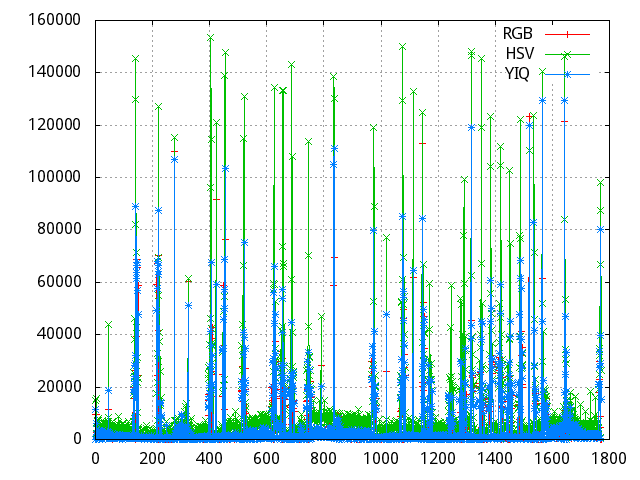
\includegraphics[scale=0.3]{02diff.png}
\caption{02.mpg frame difference}
\label{}
\end{figure}

\begin{figure}[ht]
\centering
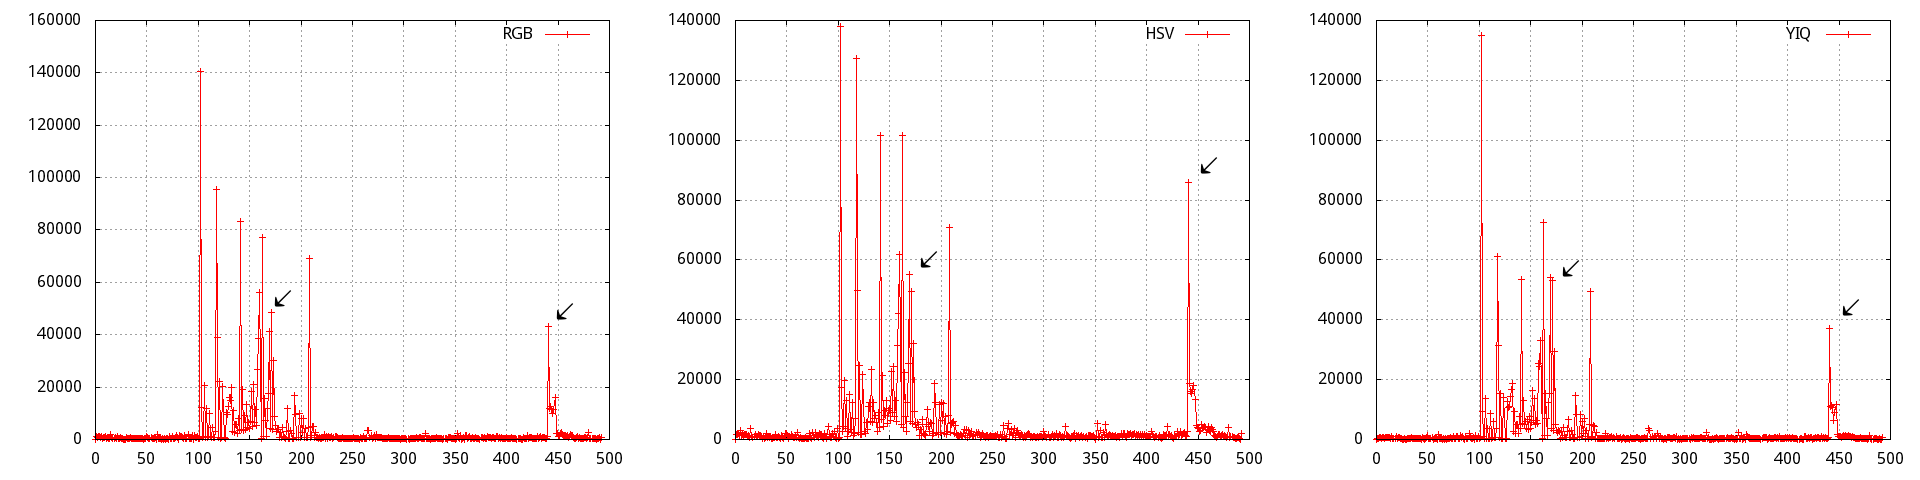
\includegraphics[scale=0.2]{03_color_space.png}
\caption{03.mpg frame difference}
\label{}
\end{figure}

\section{}
I think it's not really very well. Just need to modify the threshold for each video. But there are some transition type my program cannot detect even I use other color space, for example, 07.mpg frame 81-96.

\section{Thresholds}
\begin{CJK}{UTF8}{bkai}
除了08.mpg(多找2個,少找3個),運作非常良好,至多是多算一個或少找一個。不過如果對每個影片去挑選一個Threshold而不是共用一個Threshold的話結果會更好一點。而Threshold越高則Precision越高,Recall越低。\\
\\
我自己認為Threshold與影片的種類是相關的,我們使用Histogram來判斷是否進入另外一個Shot,是因為Histogram的變化量可以用來衡量畫面中顏色分佈的改變是否夠大,大到超過Threshold而被我們判定為這是Shot Boundary。不同主題內容種類的影像細膩的程度不同,因此發生改變的Threshold應該也會隨之有高有低。\\
\\
不過影片畫面大小有限,所以當大部分pixel發生改變的時候應該存在一個比較低的Threshold可以偵測這樣的事件,可以讓程式運作的不會太差。\\
\\
\begin{tabular}{c|c||c|c}
	\# & Threshold & Precision & Recall \\
\hline
\hline
	1 & 40000 & 1.0000 & 1.0000\\
\hline
	2 & 35000 & 1.0000 & 1.0000\\
\hline
	3 & 40000 & 0.8571 & 1.0000\\
	3 & 60000 & 1.0000 & 1.0000\\
\hline
	4 & 40000 & 0.9091 & 1.0000\\
\hline
	5 & 40000 & 1.0000 & 0.9756\\
\hline
	6 & 40000 & 1.0000 & 1.0000\\
\hline
	7 & 40000 & 1.0000 & 0.9375\\
\hline
	8 & 40000 & 0.9000 & 0.9355\\
\end{tabular}

\end{CJK}
\section{Average Shot Length}
\begin{CJK}{UTF8}{bkai}
觀察這8個影片,感覺沒什麼關聯。
\end{CJK}

\section{Representive Frame}
\begin{CJK}{UTF8}{bkai}
我認為只要簡單的挑出中間的frame作為代表的frame即可,因為在一個Shot之中大多是相似的畫面,如果這個Shot想要表達什麼,不應該放在太前面或太後面的frame出現,所以直接取中間的畫面會比較接近這個Shot的重點。\\
\\
如果取第一個frame的話可能會遇到淡入時的frame,取到一片黑色這種意味不明的frame。\\
\\
以下針對05.mpg試驗了取中間frame與取第一個frame的結果。雖然大致上看起來差不多,不過我自己覺得取中間frame的最左下那張和右下那張都比取第一個frame的還要好。\\

\begin{figure}[ht]
\centering
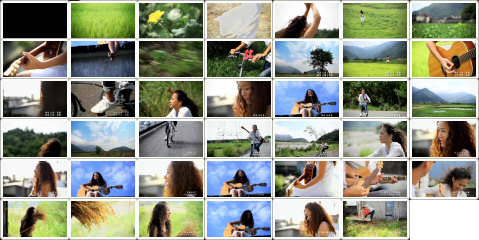
\includegraphics[scale=0.7]{first.png}
\caption{Take first frame as represent frame}
\label{}
\end{figure}

\begin{figure}[ht]
\centering
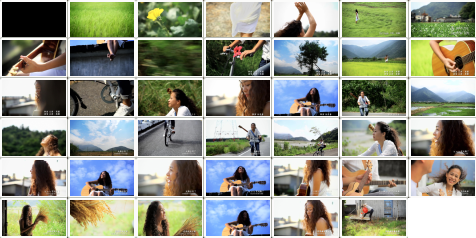
\includegraphics[scale=0.7]{middle.png}
\caption{Take middle frame as represent frame}
\label{}
\end{figure}

\end{CJK}

\end{document}
